% Figuras del informe (flotan al inicio de columna/página).
\begin{figure}[t]
\centering
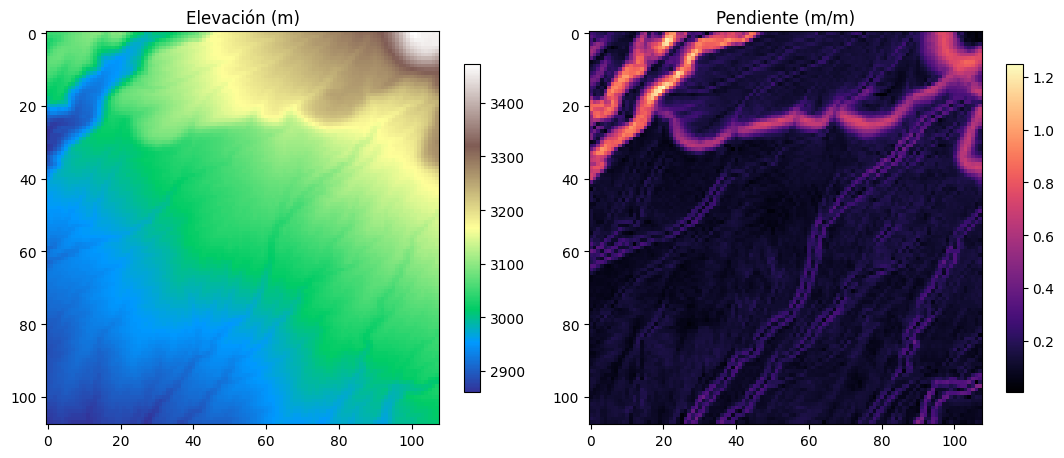
\includegraphics[width=\columnwidth]{figuras/01_terreno.png}
\caption{Terreno real (faldas del Misti): elevación (izq.) y pendiente (der.),
malla $108\times108$ de 30~m.}
\label{fig:terreno}
\end{figure}

\begin{figure}[t]
\centering
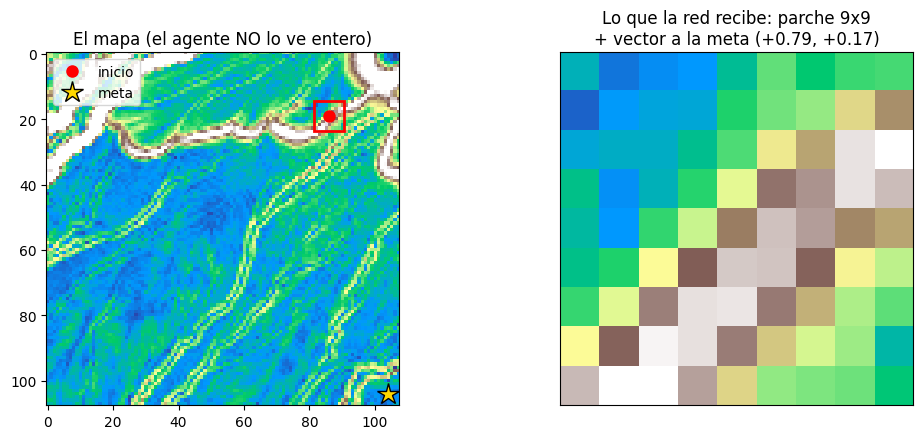
\includegraphics[width=\columnwidth]{figuras/02_observacion.png}
\caption{Observación local: el mapa completo con la ventana del agente (izq.) y el
parche $9\times9$ que recibe la red (der.), más el vector a la meta.}
\label{fig:obs}
\end{figure}

\begin{figure}[t]
\centering
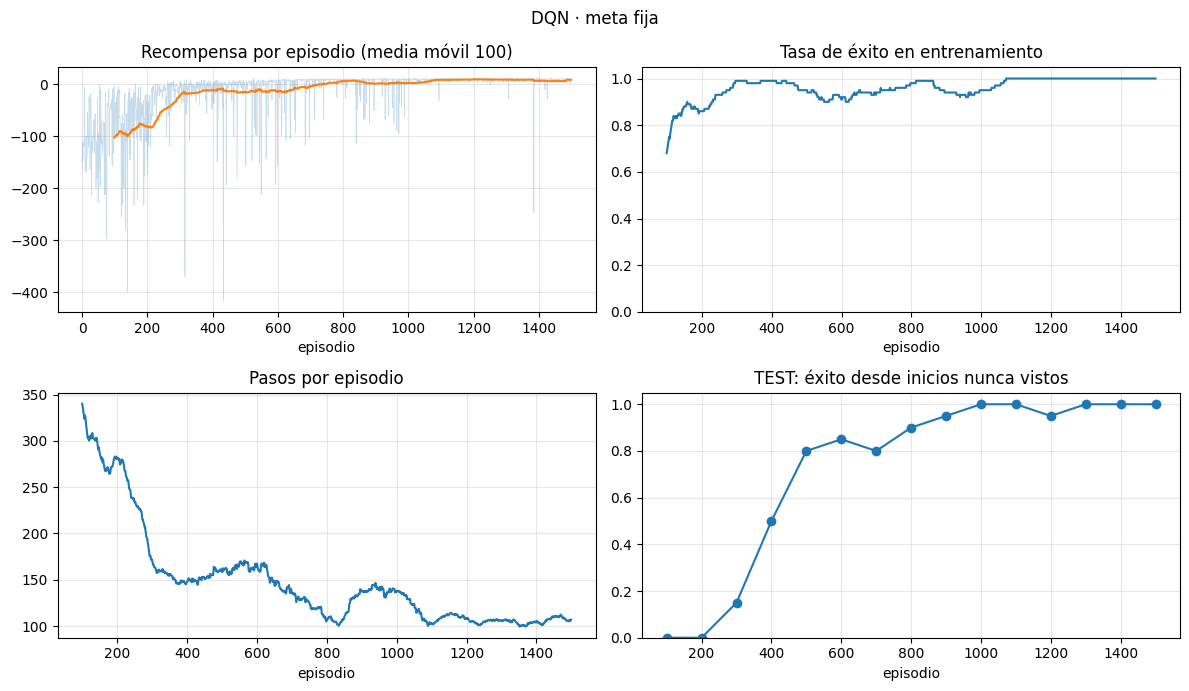
\includegraphics[width=\columnwidth]{figuras/03_curva_dqn.png}
\caption{Curva de aprendizaje de DQN con meta fija: recompensa, tasa de éxito de
entrenamiento, pasos y test sobre inicios no vistos.}
\label{fig:curva}
\end{figure}

\begin{figure}[t]
\centering
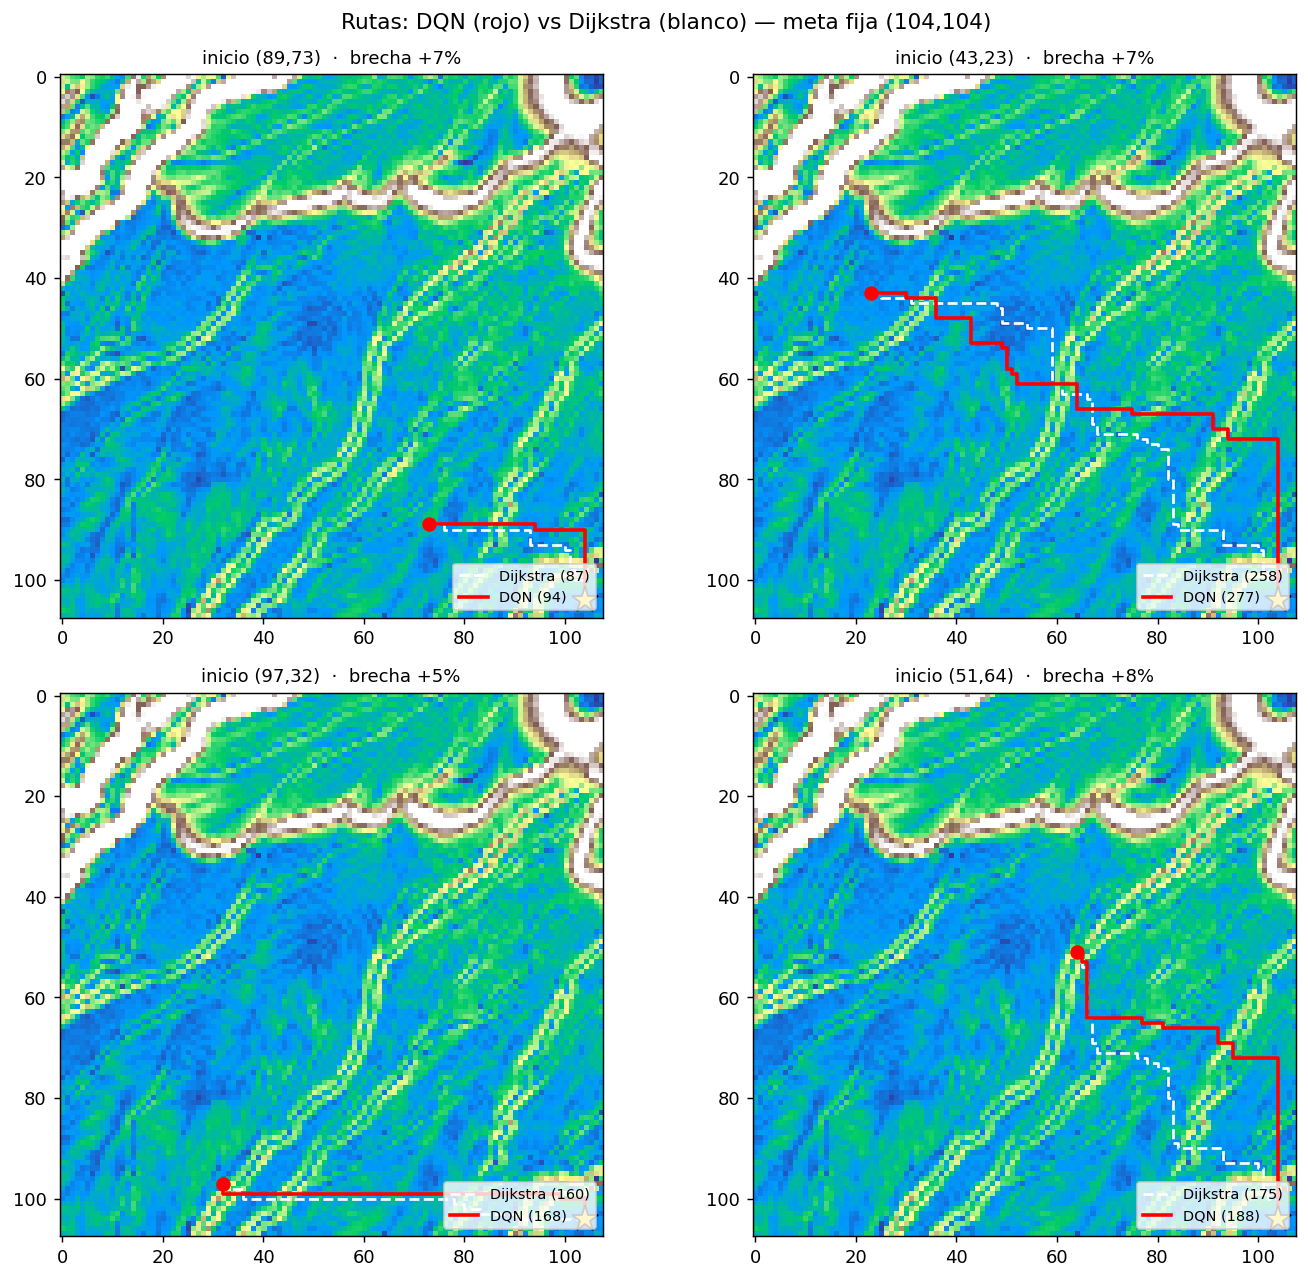
\includegraphics[width=\columnwidth]{figuras/04_rutas_dijkstra.png}
\caption{Rutas aprendidas por DQN (rojo) frente al óptimo exacto de Dijkstra
(blanco), para cuatro pares inicio--meta de test.}
\label{fig:rutas}
\end{figure}

\begin{figure}[t]
\centering
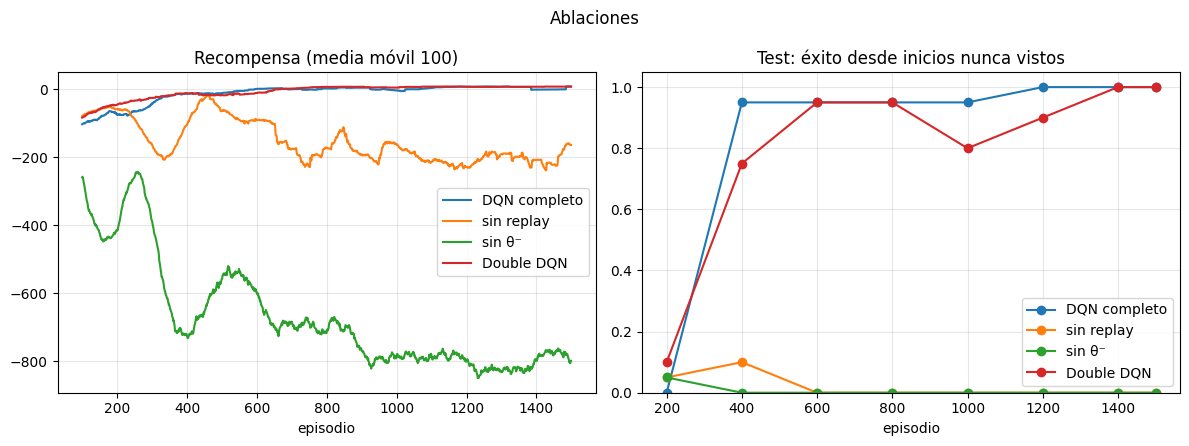
\includegraphics[width=\columnwidth]{figuras/05_ablaciones.png}
\caption{Ablaciones: DQN completo, sin \emph{replay}, sin red objetivo
($\theta^-$) y Double DQN.}
\label{fig:ablacion}
\end{figure}

\begin{figure}[t]
\centering
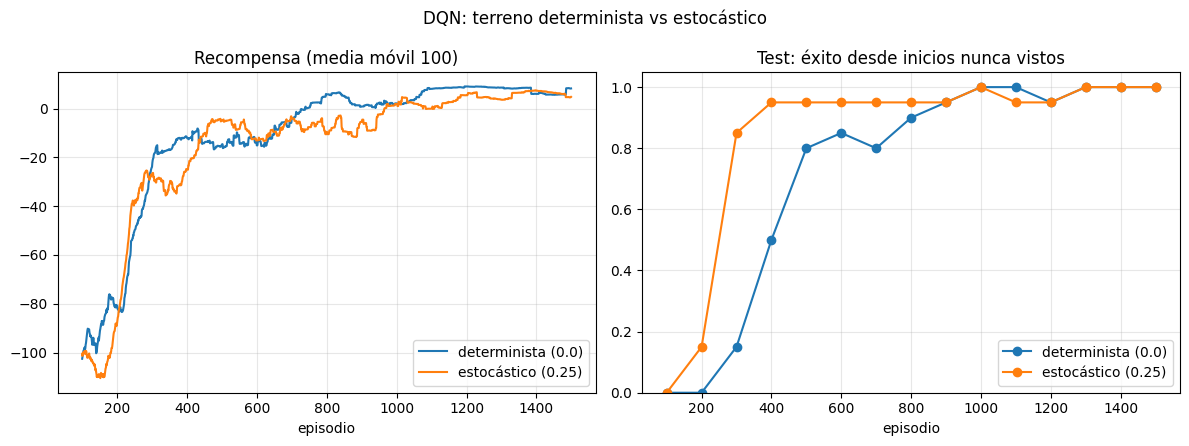
\includegraphics[width=\columnwidth]{figuras/06_estocastico.png}
\caption{DQN en terreno determinista vs estocástico (resbalón $0.25$).}
\label{fig:estoc}
\end{figure}

\begin{figure}[t]
\centering
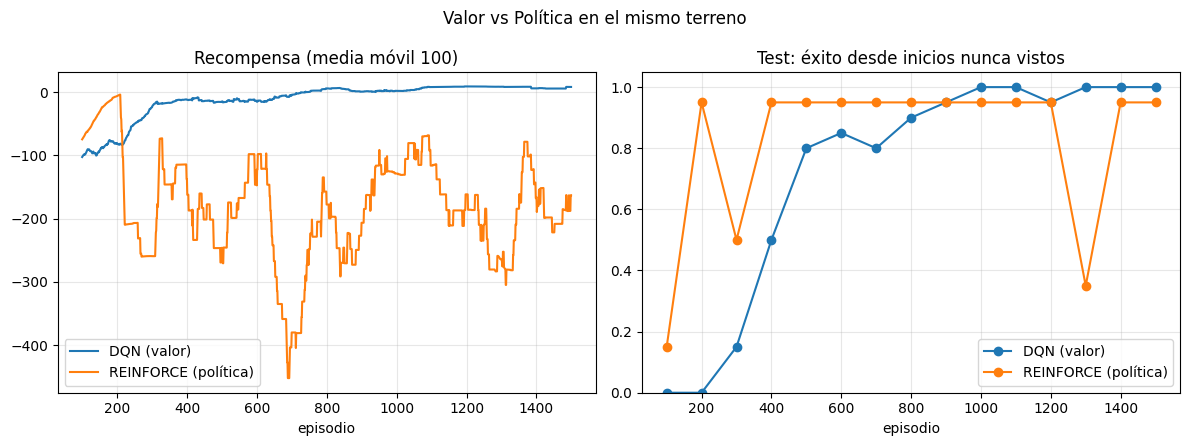
\includegraphics[width=\columnwidth]{figuras/07_dqn_vs_reinforce.png}
\caption{Valor vs política: DQN y REINFORCE en el mismo terreno.}
\label{fig:reinforce}
\end{figure}

\begin{figure}[t]
\centering
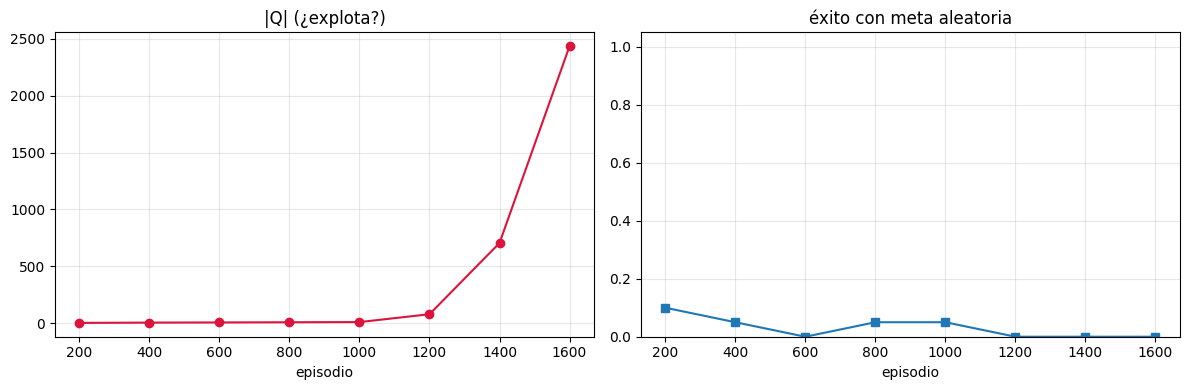
\includegraphics[width=\columnwidth]{figuras/08_divergencia.png}
\caption{Con meta aleatoria, la magnitud media de $Q$ (izq.) crece sin control
(divergencia) y el éxito (der.) no se sostiene.}
\label{fig:diverge}
\end{figure}
